\begin{figure}[h!]
\begin{center}
  \hspace*{-0.3in}
  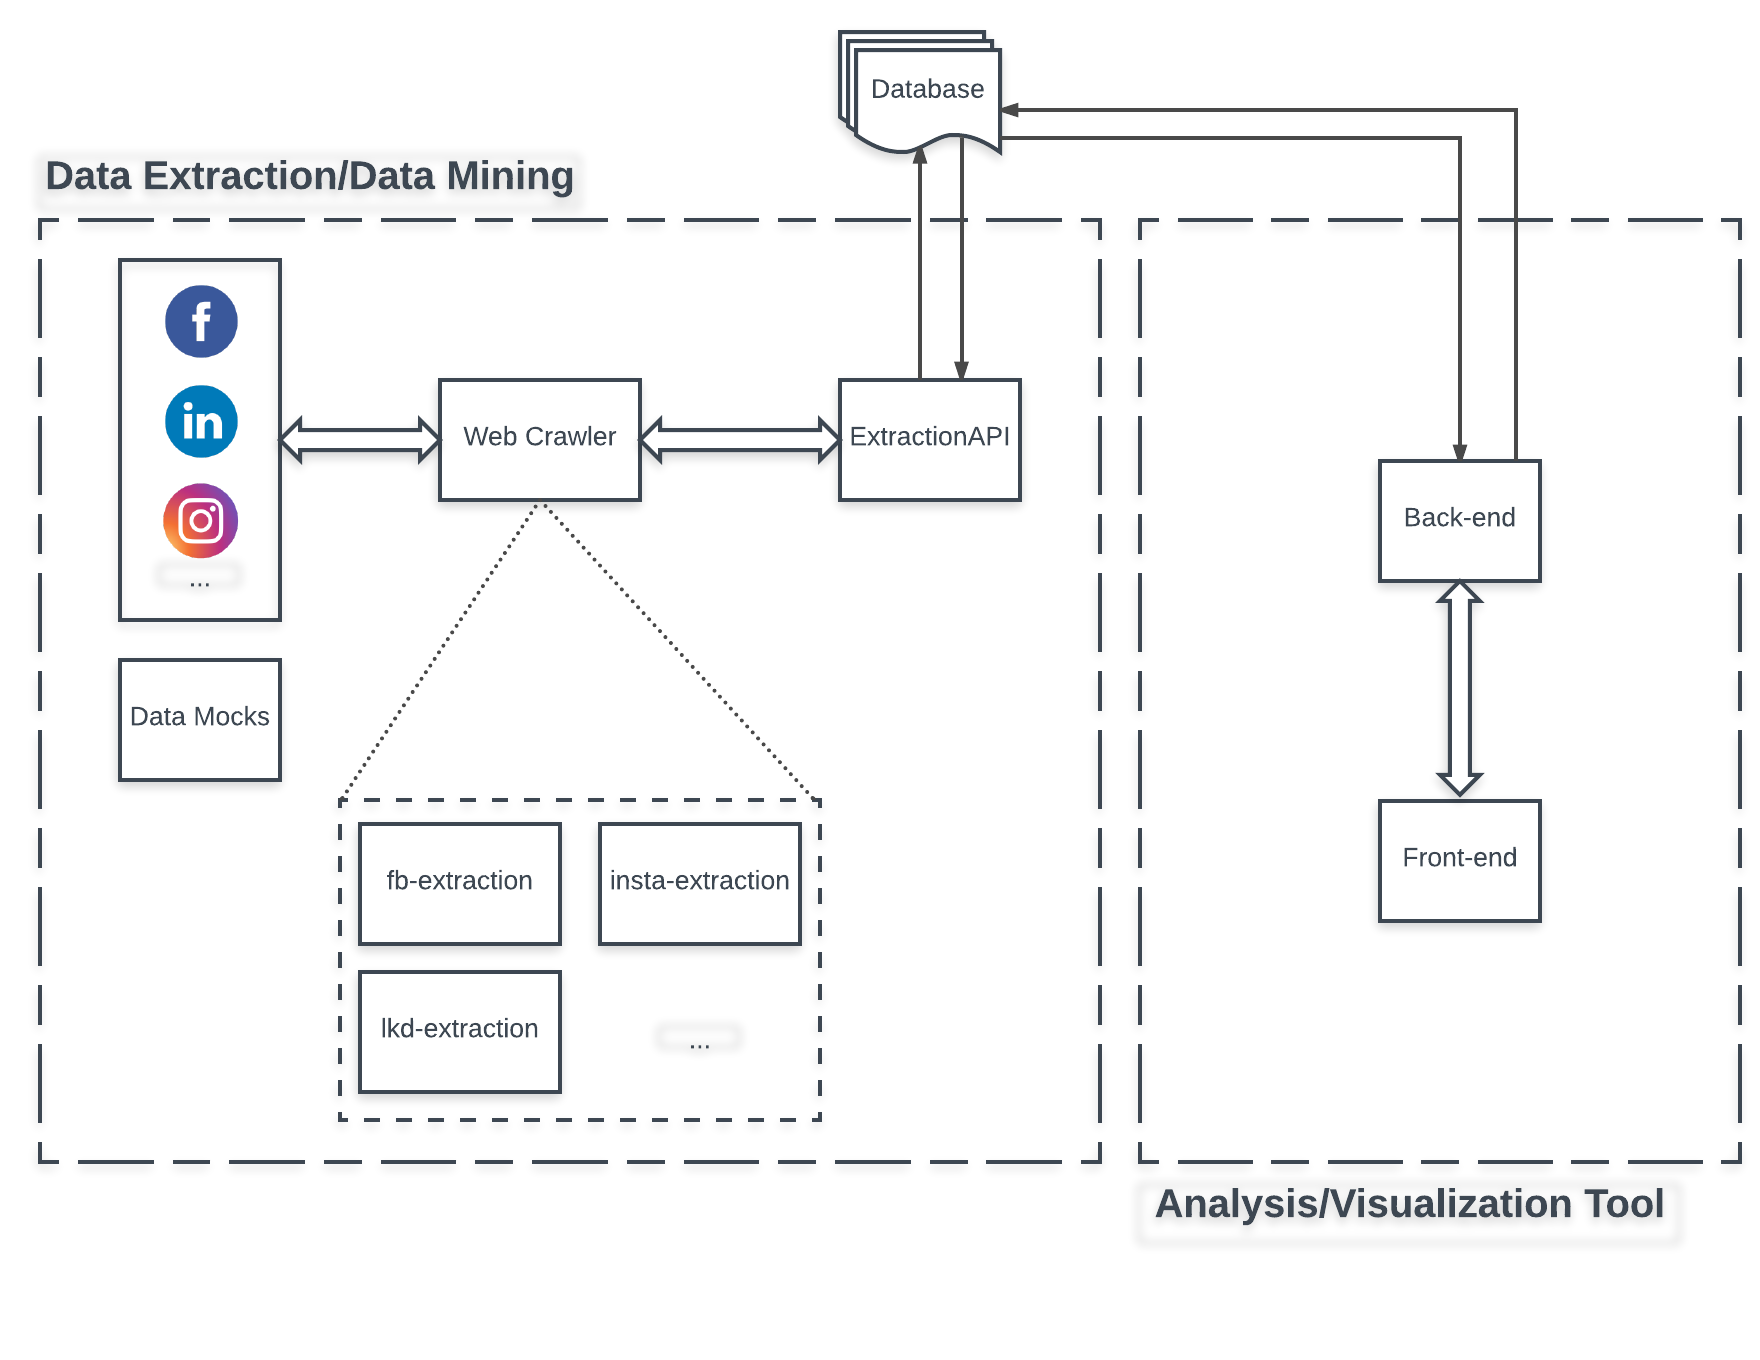
\includegraphics[width=1.1\textwidth]{img/architecture.png}
\end{center}
\caption{\label{img:architectureprop} System architecture proposal.}
\end{figure}

After exposing all the necessary theory and context on \glspl{sn} and \glspl{osn}, we know present a more concrete
image of the overall system. In Figure \ref{img:architectureprop} we present an abstract system architecture.

\subsection{General overview}
As the interaction of the software components may be clear from the diagram, the role of each module its not clear by simple
diagram observation, an underlying explanation of each component is needed in order to understand the system.\\
\indent We will follow a \textit{top down} approach for explaining the system architecture. First let us be clear about the two
main and distinct parts of the system:
\begin{itemize}
    \item \textbf{\textit{Application/Visualization and Analysis Tool}} - The tool that directly interacts with the end user
    its composed by a \textbf{Back-end} that fetches data from a database, runs calculations and algorithms on top of stored networks
    as the user requests by interacting with a \textbf{Front-end} that provides the visualization and interaction features;
    \item \textbf{\textit{Information extraction and data mining}} - All the other components are built for extract information
    from existent databases, or from \glspl{osn} (trough the \textbf{Web Crawler}) and store information being information properly treated before stored.
\end{itemize}


\subsection{Detailed Components Description}
Some of the components require a more detailed explanation, next we look more carefully into some of the components in Figure \ref{img:architectureprop}.
\begin{itemize}
    \item \textbf{\textit{Data Mocks}} - This represents the strong hypothesis that we feed some data trough data mocks, instead of crawling data from \gls{osn}. This data may be databases from projects that we already mentioned in this document, such as \cite{kunegis2013konect}. This data would be accessed trough the \textbf{Extraction API}, or a new module could be constructed exclusively to feed this data to our database;
    \item \textbf{\textit{Web Crawler}} - The \textbf{Web Crawler} consists in a set of modules for crawling each one of the \glspl{osn} (\textit{fb-extraction} and other modules);
    \item \textbf{\textit{Database}} - The database is where we store our data. It is not represented by the \textit{classical cilindro} because it resembles relational databases, and the possibility of using non relational databases such as document data bases it grows strongly within the project, and the reason is the unstructured data that we will be storing into our database.
\end{itemize}
